\documentclass[12pt,a4paper,oneside]{article}
\usepackage{graphicx,setspace,float,fancyhdr,listings,xcolor,placeins,xeCJK,tocloft,enumerate,amsmath}
\usepackage[dvipsnames]{xcolor}
\renewcommand{\cftsecleader}{\cftdotfill{\cftdotsep}} % Enable dot leaders in TOC
\renewcommand{\cftdotsep}{1} % Adjust dot spacing

\date{\Large 2024.11.11}
\author{陈海弘}

\setCJKmainfont[AutoFakeBold=3]{STFangsong} % CJK Font Setup
\setcounter{tocdepth}{3} % Set TOC depth
\setstretch{1.25} % Line spacing

% Page header and footer setup
\setlength{\headheight}{13.6pt}
\addtolength{\topmargin}{-1.6pt}
\pagestyle{fancy}
\fancyhf{}
\fancyhead[C]{\small Machine Learning} % Center header
\fancyfoot[C]{\small \thepage} % Center footer

% Code highlighting setup
\lstset{
    language=Python,
    basicstyle=\ttfamily\small,
    keywordstyle=\bfseries\color{NavyBlue},
    commentstyle=\itshape\color{red!50!green!50!blue!50},
    stringstyle=\bfseries\color{PineGreen!90!black},
    emph={self}, 
    emphstyle=\bfseries\color{Rhodamine},
    backgroundcolor=\color{black!3},
    frame=shadowbox,
    frameround=fttt,
    numbers=left,
    numberstyle=\tiny,
    stepnumber=1,
    numbersep=5pt,
    breaklines=true,
    columns=flexible,
    xleftmargin=1em,
    xrightmargin=-2em,
    aboveskip=1em,
    framexleftmargin=2em,
    escapeinside=``,
}

% Title setup
\title{
    \vspace*{-2cm}
    
\includegraphics[width=0.8\textwidth]{SYSULogo.pdf} \\[1em]
    \vfill
    \LARGE \textbf{机器学习实验报告2} \\[1em]
    \Large
    \begin{tabular}{rl}
        \textbf{姓名:} & \textbf{陈海弘} \\
        \textbf{学号:} & \textbf{23354049}
    \end{tabular}
    \vfill
}

\begin{document}
\maketitle
\newpage
\tableofcontents

\newpage
\section{摘要}
    \qquad 这次实验主要是关于逻辑回归的实验,逻辑回归是一种常用的分类算法,适用于二分类问题。在本次实验中,我们将使用逻辑回归模型对两个数据集进行分类预测。首先,我们将使用 Iris 数据集,该数据集包含了鸢尾花的花萼长度和花萼宽度等特征,以及鸢尾花的种类。我们将使用逻辑回归模型对鸢尾花的种类进行预测。其次,我们将使用 Titanic 数据集,该数据集包含了泰坦尼克号乘客的信息,以及乘客是否生还的标签。我们将使用逻辑回归模型对乘客的生还情况进行预测。在实验中,我们将实现逻辑回归模型,并使用梯度下降法训练模型,最后通过交叉验证评估模型的性能。
\section{题目}
\subsection{逻辑回归实验一}
\subsubsection{实验目的}
\qquad Iris数据集是常用的分类实验数据集,也称鸢尾花卉数据集,是一类多重变量分析的数据集。我们实验选取数据集的部分内容,包含训练集中的80个数据样本和测试集的20个样本,分为2类,每个数据包含2个属性。可通过花萼长度(x1),花萼宽度(x2)2个属性预测鸢尾花卉属于(Setosa,Versicolour)二个种类中的哪一类。

\subsubsection{数据处理}

\textbf{1.导入数据:}

首先,通过 pd.read\_csv 函数将训练数据 flower\_train.csv 和测试数据 flower\_test.csv 读取到 flower\_train 和 flower\(\)\_test 数据框中。
\newline \textbf{2.	检查缺失值:}

使用 isnull().sum() 来统计 flower\_train 中各列缺失值的数量,并输出 flower\_train 的内容。
\newline \textbf{3.	将特征 x1 和 x2 中的 0 值替换为 NaN:}

使用 replace(0, np.nan) 将 x1 和 x2 列中的所有 0 值替换为缺失值(NaN),以便后续可以更好地处理这些缺失值。
\newline \textbf{4.	用均值填充 x1 列的缺失值:}

计算每个类型 type 的 x1 列均值:

	•	首先提取 x1 列中非缺失值的行。

	•	使用 groupby 按 type 分组,并计算 x1 的均值。

	•	将结果转换成 temp 数据框,用于后续的缺失值填充。

随后,根据 type 的不同,将缺失的 x1 值替换为对应类别的均值:

	•	Iris-setosa 类型缺失的 x1 值替换为 temp['x1'][0]。

	•	Iris-versicolor 类型缺失的 x1 值替换为 temp['x1'][1]。
    \newline 	\textbf{5.	用均值填充 x2 列的缺失值:}

对 x2 列进行与 x1 类似的缺失值处理,使用每个 type 的均值填充对应的缺失值。
\newline \textbf{6.	将 type 列替换为数值表示:}

将 type 列中的字符串类型转换为数值,其中 Iris-setosa 替换为 0,Iris-versicolor 替换为 1。
\newline \textbf{7.	再次检查缺失值:}

最后,通过 isnull().sum() 查看处理后的数据框中是否还有缺失值。

\begin{lstlisting}
    # 1. 导入数据
    flower_train = pd.read_csv('flower_train.csv')
    flower_test = pd.read_csv('flower_test.csv')
    
    # 2. 检查缺失值
    print(flower_train.isnull().sum())
    
    # 3. 将 x1 和 x2 中的 0 值替换为 NaN
    flower_train[['x1', 'x2']] = flower_train[['x1', 'x2']].replace(0, np.nan)
    
    # 4. 用均值填充 x1 列的缺失值
    temp = flower_train[flower_train['x1'].notnull()]
    temp = temp[['x1', 'type']].groupby(['type'])[['x1']].mean().reset_index()
    flower_train.loc[(flower_train['type'] == 'Iris-setosa') & (flower_train['x1'].isnull()), 'x1'] = temp['x1'][0]
    flower_train.loc[(flower_train['type'] == 'Iris-versicolor') & (flower_train['x1'].isnull()), 'x1'] = temp['x1'][1]
    
    # 5. 用均值填充 x2 列的缺失值
    temp = flower_train[flower_train['x2'].notnull()]
    temp = temp[['x2', 'type']].groupby(['type'])[['x2']].mean().reset_index()
    flower_train.loc[(flower_train['type'] == 'Iris-setosa') & (flower_train['x2'].isnull()), 'x2'] = temp['x2'][0]
    flower_train.loc[(flower_train['type'] == 'Iris-versicolor') & (flower_train['x2'].isnull()), 'x2'] = temp['x2'][1]
    
    # 6. 将 type 列替换为数值表示
    flower_train['type'] = np.where(flower_train['type'] == 'Iris-setosa', 0, 1)
    
    # 7. 检查缺失值
    print(flower_train.isnull().sum())
\end{lstlisting}

结果展示:
\begin{figure}[H]
    \centering
    \begin{minipage}{0.4\textwidth}
        \centering
        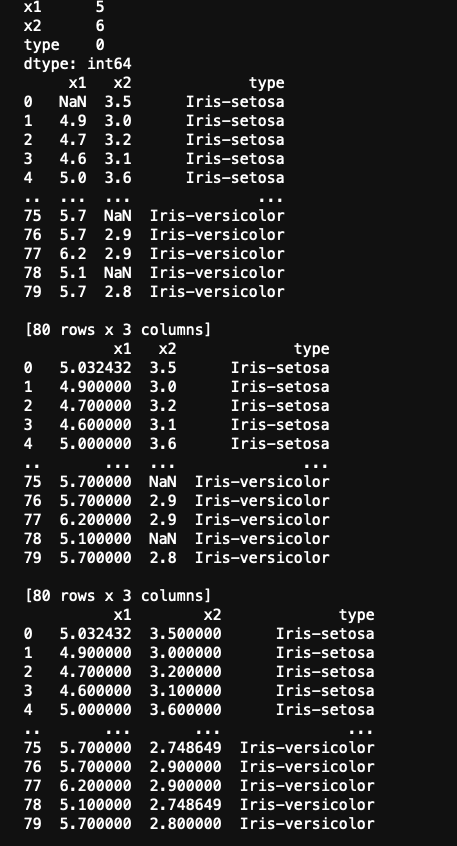
\includegraphics[width=\textwidth]{image/1} % 替换为你的图片文件名
        \caption{数据读取}
        \label{fig:image1}
    \end{minipage}
\end{figure}

\subsubsection{逻辑回归模型}

在之前的线性回归实验中,模型为$\hat{y}=\omega^T x+b$,为方便实验,该实验中将偏置量b划入模型参数中,则对应的模型变为$\hat{y}=\omega^Tx$,我们要进行相应的转换 

只需要在上一次实验中的矩阵求解析解的方法中将某一列全设置为1,即将偏置量b算入模型参数中,特征值中加入一列全1的特征量
具体实现步骤如下:

\begin{itemize}
    \item 通过 `flower\_train[['x1','x2']]` 获取训练数据的特征矩阵 $X$,并通过 `flower\_train['type']` 获取对应的目标变量 $y$。
    \item 将训练数据中的特征矩阵 $X$ 转换为 NumPy 数组,并使用 `np.hstack
    ((np.ones((X.shape[0],1)), X))` 向特征矩阵中添加一列全为 1 的列,这列对应着偏置项 $b$。
    \item 使用解析解法,求解回归系数 $\omega$:$\omega = (X^T X)^{-1} X^T y$,通过 `np.linalg.
    inv(X.T.dot(X)).dot(X.T).dot(y) 实现。
    \item 最后,输出添加了全 1 列的特征矩阵 $X$ 及计算得到的回归系数 $w$。
\end{itemize}

公式表示如下:

\[
X = \begin{bmatrix} 
1 & x_{1}^{(1)} & x_{2}^{(1)} \\
1 & x_{1}^{(2)} & x_{2}^{(2)} \\
\vdots & \vdots & \vdots \\
1 & x_{1}^{(n)} & x_{2}^{(n)} 
\end{bmatrix}
\]

\[
\hat{y} = Xw
\]

其中,$w$ 为回归系数,$w = \left( X^T X \right)^{-1} X^T y$。

\begin{lstlisting}
    x_train = flower_train[['x1','x2']].values  # 获取训练数据的特征矩阵 X
    y_train = flower_train['type'].values    # 获取训练数据的目标变量 y
    X = np.array(x_train)  
    y = np.array(y_train)
    X = np.hstack((np.ones((X.shape[0],1)),X))  # 向特征矩阵中添加一列全为 1 的列
    w = np.linalg.inv(X.T.dot(X)).dot(X.T).dot(y)
    print(X)
    print(w)
\end{lstlisting}

结果展示:
\begin{figure}[H]
    \centering
    \begin{minipage}{0.4\textwidth}
        \centering
        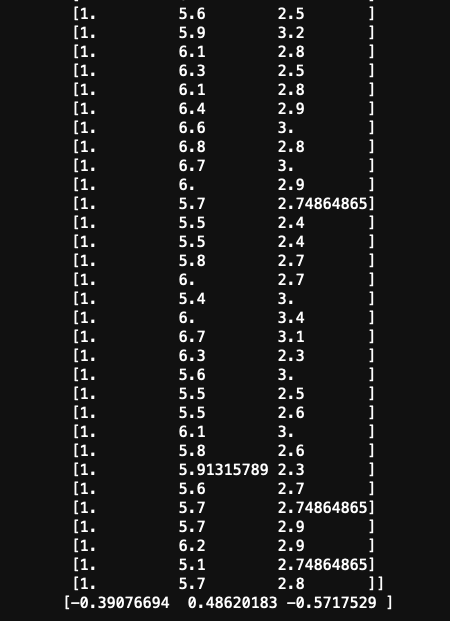
\includegraphics[width=\textwidth]{image/2} % 替换为你的图片文件名
        \caption{逻辑回归模型}
        \label{fig:image2}
    \end{minipage}
\end{figure}
可以看到,图中的第一列全为1,即为偏置项b,第二列为x1,第三列为x2,最后一行为回归系数w。

\subsubsection{手动实现梯度下降}

\qquad 由于逻辑回归的原理是用逻辑函数把线性回归的结果(-∞,∞)映射到(0,1)所以逻辑回归适合于二分类问题。我们使用sigmoid函数$g(z)=\frac{1}{1+e^{-z}}$将把线性回归的结果从(-∞,∞)映射到(0,1)。  

假设模型为线性回归模型$\hat{y}=\omega\_0+\omega\_1 x\_1+\omega\_2 x\_2+...+\omega\_n x\_n=\omega^T x$,则任意样本所对应发生的概率值函数即为$g(\hat{y})=\frac{1}{1+e^{-\hat{y}}}$,这样事情发生(定义为标签为1)的概率为
$$P(y=1|x)=\frac{1}{1+e^{-\omega^T x}}$$  

对应于任意一个样本(${x_i}$,$y_i$),其中$x_i$为特征值,$y_i$为实际结果值,在参数$\omega$下,该样本发生的概率为
$$P(y_i|x_i,\omega)=y_i{P(y_i=1|x_i)}+({1-y_i}){P(y_i=0|x_i)}$$

将每个样本发生概率相乘,得到似然函数:
$$\Pi^m_{i=1}{P(y_i|x_i,\omega)}$$

为了计算方便,一般取对数得到对数似然函数:
$$L(\omega)=\sum^m_{i=1}{lnP(y_i|x_i,\omega)}$$  

我们总是希望出现预测正确的概率的可能性最大,即想要得到极大化似然函数对应的参数$\omega$。这样最大化似然函数就转变为最小化似然函数的负数,取负的平均对数似然函数为损失函数,通过这样构建的损失函数
\begin{equation*}
    \begin{split}
    J(\omega) &= -\frac{1}{m}\sum^m_{i=1}{lnP(y_i|x_i,\omega)} \\
    &= -\frac{1}{m}\sum^m_{i=1}ln\Big(y_i\frac{1}{1+e^{-\omega^T x_i}} \\
    &\quad\quad\quad\quad\quad + (1-y_i)\frac{e^{-\omega^T x_i}}{1+e^{-\omega^T x_i}}\Big)
    \end{split}
    \end{equation*}





    \subsubsection{逻辑回归模型训练}

    \qquad 在本次实验中,我们使用梯度下降法训练逻辑回归模型。逻辑回归模型的目标是通过最大化似然函数来找到最优的参数 $\omega$。由于逻辑回归的输出是一个概率值,其值在 $(0, 1)$ 范围内,因此我们通过使用 Sigmoid 函数将线性回归的输出映射到该范围。
    \newline\textbf{Sigmoid 函数}

    Sigmoid 函数的定义为:
    \[
    g(z) = \frac{1}{1 + e^{-z}}
    \]
    它将任意实数 $z$ 映射到 $(0, 1)$ 范围内,适用于处理二分类问题。在逻辑回归中,模型的预测值 $\hat{y}$ 是一个基于特征输入 $x$ 的线性组合,我们通过 Sigmoid 函数将其映射为概率值。
    \newline\textbf{损失函数}

    逻辑回归模型的损失函数通常是对数损失函数(Log Loss),它衡量模型预测与实际标签之间的差异。给定特征矩阵 $X$ 和实际标签 $y$,损失函数为:
    \[
    L(\omega) = -\frac{1}{m} \sum_{i=1}^{m} \left[ y_i \ln(\hat{y}_i) + (1 - y_i) \ln(1 - \hat{y}_i) \right]
    \]
    其中,$m$ 为样本数量,$y_i$ 为样本 $i$ 的实际标签,$\hat{y}_i = g(X_i \cdot \omega)$ 为模型的预测值。
    \newline\textbf{梯度计算}

    为了最小化损失函数,我们需要计算损失函数相对于模型参数 $\omega$ 的梯度。梯度的计算如下:
    \[
    \frac{\partial L(\omega)}{\partial \omega} = \frac{1}{m} X^T (g(X \omega) - y)
    \]
    其中,$g(X \omega)$ 是模型的预测值,$y$ 是实际标签。
    \newline\textbf{梯度下降法}

    梯度下降法是一种优化算法,用于通过迭代更新模型参数 $\omega$,使损失函数最小化。每次迭代时,我们按照以下公式更新参数:
    \[
    \omega := \omega - \eta \cdot \frac{\partial L(\omega)}{\partial \omega}
    \]
    其中,$\eta$ 是学习率,控制每次更新的步长。
    \newline\textbf{模型训练过程}

    在每次迭代中,我们首先计算损失函数值,然后计算梯度,最后根据梯度更新参数 $\omega$。迭代次数设定为 1000 次,每 100 次打印一次损失值。
    
    \[
    \omega = \text{初始化为零}
    \]
    \[
    \text{每 100 次打印损失值}
    \]
    \newline\textbf{Python 实现}
      
    通过以下 Python 代码实现梯度下降法训练逻辑回归模型:
    
    \begin{lstlisting}  
# 定义 Sigmoid 函数
def sigmoid(z):
    return 1 / (1 + np.exp(-z))

# 计算损失函数 J($\omega$)
def compute_loss(X, y, w):
    m = len(y)
    y_hat = sigmoid(X.dot(w))  # 预测值
    loss = -np.mean(y * np.log(y_hat) + (1 - y) * np.log(1 - y_hat))
    return loss

# 计算梯度
def compute_gradient(X, y, w):
    m = len(y)
    y_hat = sigmoid(X.dot(w))
    gradient = (1 / m) * X.T.dot(y_hat - y)
    return gradient

# 梯度下降法训练逻辑回归模型
def logistic_regression(X, y, learning_rate=0.01, num_iterations=1000):
    # 初始化模型参数 $\omega$
    w = np.zeros(X.shape[1])

    # 迭代更新参数
    for i in range(num_iterations):
        gradient = compute_gradient(X, y, w)  # 计算梯度
        w = w - learning_rate * gradient      # 更新权重
        # 打印每 100 次迭代的损失
        if i % 100 == 0:
            loss = compute_loss(X, y, w)
            print(f"Iteration {i}, Loss: {loss}")

    return w

# 训练模型
learning_rate = 0.1
num_iterations = 1000
w = logistic_regression(X, y, learning_rate, num_iterations)

print("Trained weights:", w)

    \end{lstlisting}
    
    通过梯度下降法的迭代优化,我们得到了最优的参数 $\omega$,从而完成了逻辑回归模型的训练过程。

    \begin{figure}[H]
        \centering
        \begin{minipage}{0.4\textwidth}
            \centering
            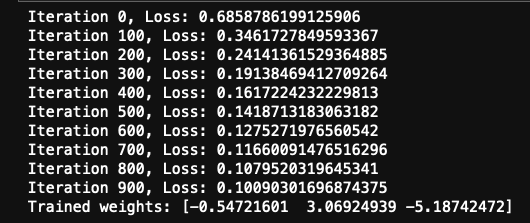
\includegraphics[width=\textwidth]{image/3} % 替换为你的图片文件名
            \caption{训练结果}
            \label{fig:image3}
        \end{minipage}
    \end{figure}
    \subsubsection{损失函数计算}
    在模型训练完成后得到所训练的模型参数$\omega$,在测试集上进行所训练模型的测试并使用之前所介绍的损失函数计算loss值

    \begin{lstlisting} 
        X_test = np.hstack([np.ones((X_test.shape[0], 1)), X_test])  # Add bias column if needed
        y_pred_prob = sigmoid(X_test.dot(w))
        compute_loss(X_test, y_pred_prob, w)
    \end{lstlisting}

    \subsubsection{逻辑回归模型预测}
    \qquad 要输出可视化结果,首先画出决策边界,然后将训练集和测试集的数据点绘制在图中。决策边界是指模型预测为正类和负类的分界线,即预测概率为 0.5 的位置。
    
    1.	设置图像和网格范围:定义图像尺寸和x、y轴的范围,为决策边界和数据点提供展示区域。
	
    2.	生成网格点:在x、y轴范围内生成密集的网格点,便于在整个图上绘制决策边界。
	
    3.	添加偏置项:为每个网格点的特征添加偏置项,使其符合逻辑回归模型参数的格式。
	
    4.	定义模型参数:假设一个逻辑回归模型的参数(包含偏置和权重)用于预测。
	
    5.	计算预测值:使用逻辑回归模型,对网格点进行预测,得到每个点的类别(0或1),形成决策边界的分类区域。
	
    6.	绘制决策边界:根据预测结果填充决策边界区域,直观地展示模型对不同区域的分类情况。
	
    7.	绘制数据点:用不同颜色标记数据集中各类样本点,显示在图中与决策边界的关系。

    \begin{lstlisting}
        w = np.array([[0], [3], [-6]])
        z = grid.dot(w)
        for i in range(len(z)): 
            z[i][0] = (1 / (1 + np.exp(-z[i])))
            z[i][0] = 0 if z[i][0] < 0.5 else 1     #如果预测值小于0.5则预测为0,否则预测为1
    \end{lstlisting}

    \begin{figure}[H]
        \centering
        \begin{minipage}{0.4\textwidth}
            \centering
            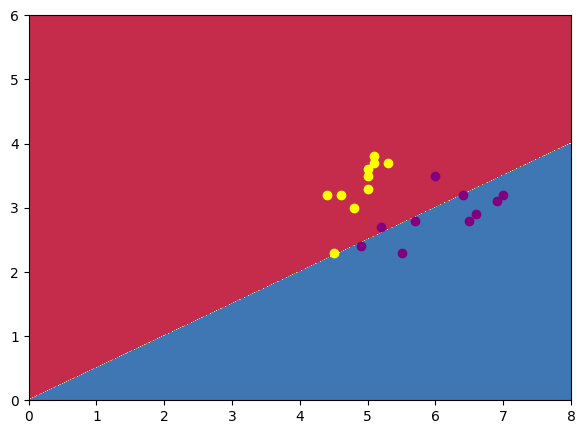
\includegraphics[width=\textwidth]{image/4} % 替换为你的图片文件名
            \caption{预测结果}
            \label{fig:image4}
        \end{minipage}
    \end{figure}

    可以看到,图中的蓝色区域表示模型预测为 0 的区域,黄色区域表示模型预测为 1 的区域,决策边界为两个区域的分界线。数据点的颜色表示实际的类别,紫色点为类别 0,黄色点为类别 1。逻辑回归模型通过学习训练数据,得到了较好的分类效果。
\subsection{逻辑回归实验二}
\subsubsection{实验目的}

\qquad 该数据集(trai\_titanic.csv和test\_titanic.csv)同样为分类数据集,为泰坦尼克号的乘客信息以及最后是否生还。包括了七个特征值以及一个类别特征(即为Survived类型,代表是否生还),特征信息分别为Passengerid(乘客id),Age(乘客年龄),Fare(船票价格),Sex(性别),sibsp(堂兄弟妹个数),Parch(父母与小孩的个数),Pclass(乘客等级)

观察到有七个特征值,并且数据集都做了处理,没有缺失值,字符串都是整数类型,但是七个特征值和最后是否生还的关联度不同,所以可以选择两次,每一次随机选择四个特征值,然后进行十次十折交叉验证,最后得到最好的特征值组合,然后再进行逻辑回归模型的训练。

\subsubsection{数据读取}
\qquad 使用pandas库的read\_csv函数读取训练数据集和测试数据集,查看数据集的前几行,以及数据集的基本信息。
\begin{lstlisting}
    train_data = pd.read_csv('train_titanic.csv')
    test_data = pd.read_csv('test_titanic.csv')
    print(train_data.head())
    print(test_data.head())
\end{lstlisting}

\subsubsection{逻辑回归模型训练}

\qquad 做两次,每次选择四个特征值建立逻辑回归模型,然后利用梯度下降方法,因为数据集样本数量较大,使用随机梯度下降法或者是小批量梯度下降法进行模型训练,最后利用十次十折交叉验证模型的准确率,选择最好的特征值组合。
\newline\textbf{1. 数据加载与预处理}

	•	使用 pandas 读取 Titanic 数据集(train\_titanic.csv)。
	•	提取特征和目标变量:
	•	第一段代码选择了特征 ['Passengerid', 'Fare', 'Age', 'Sex']。
	•	第二段代码选择了特征 ['Sex', 'sibsp', 'Parch', 'Pclass']。
	•	将特征矩阵和目标变量分别存储为 X 和 y,用于后续训练。
    \newline\textbf{2. 逻辑回归的实现}

(1) Sigmoid 函数

	•	定义了 Sigmoid 函数,公式为:

$\sigma(z) = \frac{1}{1 + e^{-z}}$

它将线性输出映射为 [0, 1] 的概率值。

(2) 损失函数

	•	使用交叉熵损失衡量模型的预测效果:

$J(\theta) = -\frac{1}{m} \sum_{i=1}^m \left[y_i \log(y_{pred}) + (1 - y_i) \log(1 - y_{pred})\right]$


(3) 梯度下降优化

	•	使用随机梯度下降(SGD)和小批量(Mini-Batch)梯度下降优化模型参数 $\theta$。

	•	每次迭代中:

	1.	打乱数据顺序以避免顺序偏差。

	2.	按批量大小(batch\_size)对数据进行分割。

	3.	计算预测值 y\_pred 和梯度,并更新参数 $\theta$。

	4.	重复多个 epoch。
\newline\textbf{3. 模型预测}

	•	根据模型参数 $\theta$,利用 Sigmoid 函数对测试数据进行预测:

\text{Prediction} =
$\begin{cases}
1, & \text{if } \sigma(z) \geq \text{threshold} \\
0, & \text{otherwise}
\end{cases}$
\newline\textbf{4. 交叉验证}

(1) 目的

	•	使用 K 折交叉验证(10 折)评估模型的泛化能力,重复多次以减少随机性。

(2) 实现

	1.	使用 KFold 将数据分为训练集和验证集。

	2.	对每一折训练:

	•	使用训练集训练逻辑回归模型。

	•	在验证集上评估模型的准确率。

	3.	重复 iterations 次,记录所有折的平均准确率。

	4.	保存具有最高平均准确率的模型参数。
\newline\textbf{5. 输出结果}

	•	打印模型在交叉验证中的最佳准确率(best\_accuracy)。
	•	打印对应的最优参数(best\_theta)。

关键点

	•	实验目标:实现逻辑回归模型,预测 Titanic 乘客的生存情况。

	方法:

	•	使用随机梯度下降优化参数。

	•	利用 10x10 折交叉验证评估模型性能。

	•	评估指标:模型在验证集上的准确率。

	结论:

	•	代码分别尝试了不同的特征组合,分析其对预测结果的影响。

	•	通过交叉验证,找到了最优参数和最佳模型性能。

    \begin{lstlisting}
        import numpy as np
        import pandas as pd
        from sklearn.model_selection import KFold
        
        # Load data
        train_data = pd.read_csv('train_titanic.csv')
        X = train_data[['Passengerid', 'Fare', 'Age', 'Sex']].values
        y = train_data['Survived'].values
        
        # Sigmoid function
        def sigmoid(z):
            return 1 / (1 + np.exp(-z))
        
        # Compute loss
        def compute_loss(y, y_pred):
            m = y.shape[0]
            return -np.sum(y * np.log(y_pred) + (1 - y) * np.log(1 - y_pred)) / m
        
        # SGD/Mini-Batch Gradient Descent function
        def gradient_descent(X, y, batch_size=32, learning_rate=0.01, epochs=100):
            m, n = X.shape
            theta = np.zeros(n)
            for epoch in range(epochs):
                # Shuffle data for each epoch
                indices = np.arange(m)
                np.random.shuffle(indices)
                X = X[indices]
                y = y[indices]
                
                # Mini-batch gradient descent
                for i in range(0, m, batch_size):
                    X_batch = X[i:i + batch_size]
                    y_batch = y[i:i + batch_size]
                    
                    # Predictions and gradients
                    z = np.dot(X_batch, theta)
                    y_pred = sigmoid(z)
                    gradient = np.dot(X_batch.T, (y_pred - y_batch)) / batch_size
                    theta -= learning_rate * gradient
        
            return theta
        
        # Prediction function
        def predict(X, theta, threshold=0.5):
            return (sigmoid(np.dot(X, theta)) >= threshold).astype(int)
        
        # Cross-validation with 10x10-fold
        def cross_validate(X, y, k=10, iterations=10):
            best_accuracy = 0
            best_theta = None
            
            for _ in range(iterations):
                kf = KFold(n_splits=k, shuffle=True, random_state=1)
                accuracies = []
        
                for train_index, val_index in kf.split(X):
                    X_train, X_val = X[train_index], X[val_index]
                    y_train, y_val = y[train_index], y[val_index]
                    
                    # Train with mini-batch gradient descent
                    theta = gradient_descent(X_train, y_train)
                    
                    # Evaluate on validation set
                    y_pred = predict(X_val, theta)
                    accuracy = np.mean(y_pred == y_val)
                    accuracies.append(accuracy)
        
                avg_accuracy = np.mean(accuracies)
                
                # Track the best theta based on accuracy
                if avg_accuracy > best_accuracy:
                    best_accuracy = avg_accuracy
                    best_theta = theta
                    
            return best_theta, best_accuracy
        
        # Run cross-validation
        best_theta1, best_accuracy1 = cross_validate(X, y)
        print(f"Best Accuracy1 from Cross-Validation: {best_accuracy1}")
        print("Best Model1 Parameters (Theta):", best_theta1)
        
        
        X = train_data[['Pclass', 'Fare', 'Age', 'Sex']].values
        best_theta2, best_accuracy2 = cross_validate(X, y)
        print(f"Best Accuracy2 from Cross-Validation: {best_accuracy2}")
        print("Best Model2 Parameters (Theta):", best_theta2)
    \end{lstlisting}
    \begin{figure}[H]
        \centering
        \begin{minipage}{0.7\textwidth}
            \centering
            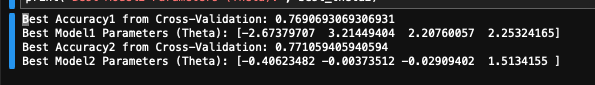
\includegraphics[width=\textwidth]{image/5} % 替换为你的图片文件名
            \caption{训练结果}
            \label{fig:image5}
        \end{minipage}
    \end{figure}
    \subsubsection{模型预测}实验步骤:

    1.	加载数据:读取测试集数据,提取特征(Pclass、Fare、Age、Sex)和目标变量(Survived)。
	
    2.	预测:使用训练好的模型(best\_theta2),通过 Sigmoid 函数计算概率,并根据设定的阈值(0.2)将概率转换为二分类标签(0或1)。
	
    3.	评估性能:
	
    •	计算 准确率、精确率 和 召回率。
	
    4.	绘制曲线:
	
    •	绘制 Precision-Recall 曲线,分析精确率和召回率的权衡。
	
    •	绘制 ROC 曲线,分析假正例率与真正例率的关系,并计算 AUC(曲线下的面积)。
	
    5.	优化阈值:通过调整阈值来平衡精确率和召回率,提升模型性能。

    \begin{lstlisting}
        #your code here------
        import numpy as np
        import pandas as pd
        from sklearn.metrics import accuracy_score, precision_score, recall_score, roc_curve, auc, precision_recall_curve
        import matplotlib.pyplot as plt
        
        # Load the test data
        test_data = pd.read_csv('test_titanic.csv')
        X_test = test_data[['Pclass', 'Fare', 'Age', 'Sex']].values
        y_test = test_data['Survived'].values
        
        
        # Predict function (reusing the trained model's best_theta)
        y_test_pred_proba = sigmoid(np.dot(X_test, best_theta2))  # Probability predictions
        y_test_pred = (y_test_pred_proba >= 0.2).astype(int)     # Binary predictions (0 or 1)
        
        # Calculate Metrics
        accuracy = accuracy_score(y_test, y_test_pred)
        precision = precision_score(y_test, y_test_pred)
        recall = recall_score(y_test, y_test_pred)
        
        print("Test Accuracy:", accuracy)
        print("Test Precision:", precision)
        print("Test Recall:", recall)
        
        # Plot Precision-Recall Curve
        precision_vals, recall_vals, _ = precision_recall_curve(y_test, y_test_pred_proba)
        plt.figure(figsize=(8, 6))
        plt.plot(recall_vals, precision_vals, marker='.')
        plt.xlabel('Recall')
        plt.ylabel('Precision')
        plt.title('Precision-Recall Curve')
        plt.show()
        
        # Plot ROC Curve
        fpr, tpr, _ = roc_curve(y_test, y_test_pred_proba)
        roc_auc = auc(fpr, tpr)
        plt.figure(figsize=(8, 6))
        plt.plot(fpr, tpr, label=f'ROC Curve (AUC = {roc_auc:.2f})')
        plt.plot([0, 1], [0, 1], 'k--', label='Random Classifier')
        plt.xlabel('False Positive Rate')
        plt.ylabel('True Positive Rate')a
        plt.title('ROC Curve')
        plt.legend()
        plt.show()
    \end{lstlisting}

实验结果:
\textbf{\\
Test Accuracy: 0.76\\
Test Precision: 0.6944444444444444\\
Test Recall: 0.6578947368421053}
可以看到,模型在测试集上的准确率为 0.76,精确率为 0.69,召回率为 0.66。通过绘制 Precision-Recall 曲线和 ROC 曲线,我们可以更直观地分析模型的性能。\\

\begin{figure}[H]
    \centering
    \begin{minipage}{0.5\textwidth}
        \centering
        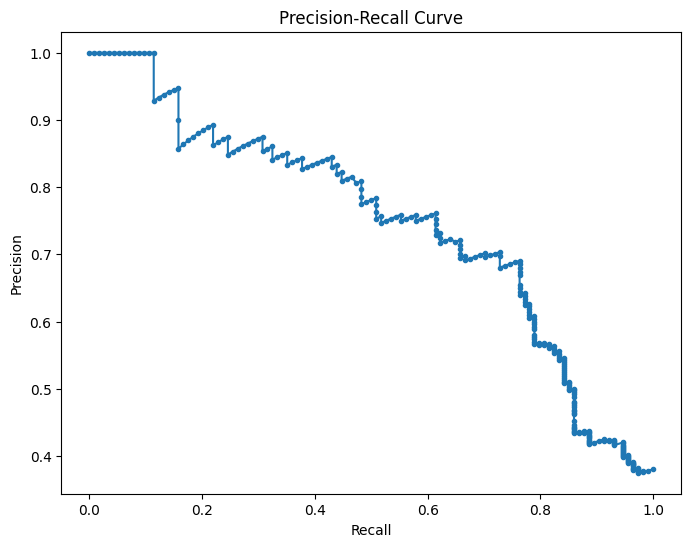
\includegraphics[width=\textwidth]{image/PR} % 替换为你的图片文件名
        \caption{PR}
        \label{fig:image6}
    \end{minipage}
    \begin{minipage}{0.5\textwidth}
        \centering
        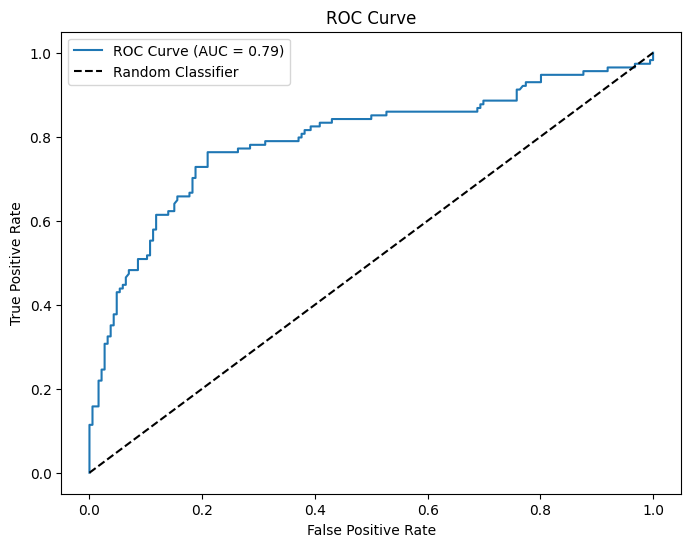
\includegraphics[width=\textwidth]{image/RC} % 替换为你的图片文件名
        \caption{ROC}
        \label{fig:image7}
    \end{minipage}
\end{figure}

PR图展示了精确率和召回率之间的权衡,其中,横轴为召回率,纵轴为精确率。图形越靠近右上角,模型性能越好。

ROC图展示了假正例率和真正例率之间的关系,其中,横轴为假正例率,纵轴为真正例率。曲线下的面积(AUC)越大,模型性能越好。而图中的虚线表示随机分类器的性能,即 AUC=0.5。

\section{总结}
\qquad 本次实验主要学习了逻辑回归模型的原理和实现方法,通过两个实验分别对鸢尾花数据集和泰坦尼克号数据集进行了逻辑回归模型的训练和预测。在实验一中,我们通过解析解法和梯度下降法训练了逻辑回归模型,并对模型的性能进行了评估。在实验二中,我们通过交叉验证选择了最佳特征组合,并在测试集上评估了模型的性能。通过实验,我们掌握了逻辑回归模型的基本原理和实现方法,以及如何使用交叉验证评估模型性能。逻辑回归模型是一种简单而有效的分类模型,适用于二分类问题,具有较好的解释性和可解释性,是机器学习中常用的模型之一。

\end{document}
